%========================================================
%Arquitectura de Proceso
%========================================================

%========================================================
%Revisión
%-------------------------------------------

% \UCccitem{Versión}{1}
% \UCccsection{Análisis de Procesos }
% \UCccitem{Autor}{nombreAutor}
% \UCccitem{Evaluador}{nombreEvaluador}
% \UCccitem{Prioridad}{Alta} %Alta, media, baja
% \UCccitem{Estatus}{} %Edición, Terminado, Corrección, Aprobado 
% \UCccitem{Complejidad}{Alta} %Alta, Media, Baja
% \UCccitem{Volatilidad}{Alta} %Alta, Media, Baja
% \UCccitem{Madurez}{Media}  %Alta, Media, Baja
% \UCccsection{Control de cambios}
% \UCccitem{Versión 0}{
% \begin{UClist}
% \RCitem{ Pxn T1}{Corregir la ortografía}{\DONE}
% \TODO es para solicitar un cambio, \TOCHK Es para informar que se atendió el TODO, \DONE Es para indicar que el evaluador reviso los cambios.
% \end{UClist}
%}

%Organigrama

%	\begin{figure}[hbtp!]
%		\begin{center}
%			\fbox{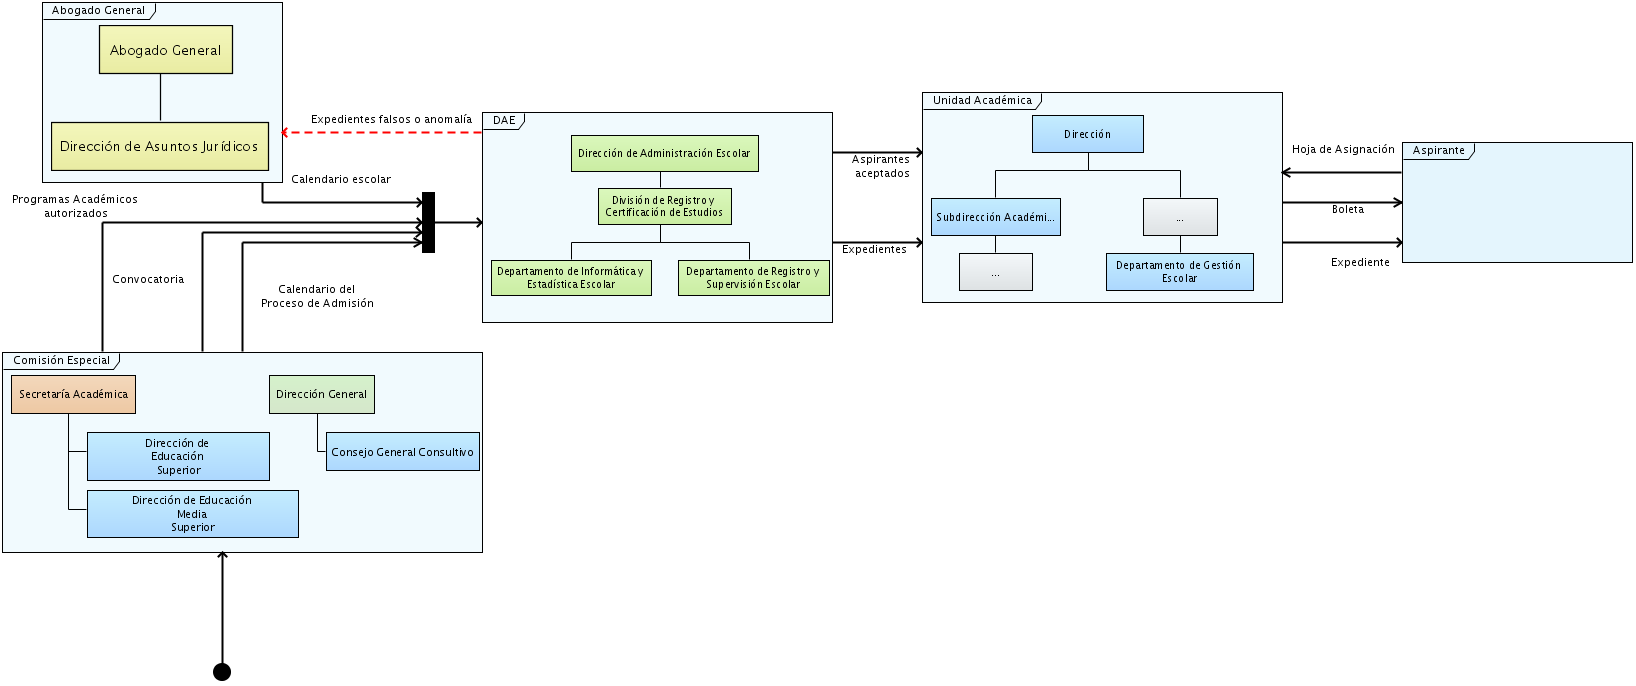
\includegraphics[width=\textwidth]{pin/imagenes/INT-IN-Inscripcion}}
%			\caption{Interacción de Áreas}
%		\end{center}
%		
%	\end{figure}

%========================================================
% Descripción general del proceso
%-----------------------------------------------
\begin{Arquitectura}{AG-IN}{Arquitectura del Proceso de Ingreso} {
		
	%-------------------------------------------
	%Descripción
	El Proceso de Ingreso corresponde al mecanismo por medio del cual un \refElem{Aspirante}, que realizó todos los trámites correspondientes al \textbf{Proceso de Admisión} y fue seleccionado para pertenecer a una unidad académica se convierte en \refElem{Alumno} del Instituto. El alumno es el centro de la vida académica y el principal usuario de todos los servicios que ofrece el Instituto. 
	
	La figura \cdtRefImg{arq:AG-IR}{AG-IR Proceso de ingreso} muestra la interacción con los procesos que proporcionan la información necesaria para llevar a cabo sus funciones. Este proceso, está vinculado con distintos procesos y distintas áreas de las cuales obtiene información referente a: La estructura académica correspondiente al periodo que se iniciará, tiempos de los procesos y aspirantes aceptados. En caso en que un aspirante haya incumplido en alguno de los artículos que se encuentran en el Reglamento General de Estudios y en la Convocatoria Correspondiente se anulará su proceso de ingreso. En la siguiente sección se detalla esta interacción.
		\Pfig[0.8]{pin/imagenes/ArqPG-IN-Ingreso}{arq:AG-IN}{AG-IN Proceso de ingreso.}		
	}{AG-IN}

\end{Arquitectura}

%========================================================
%Interacción
%-----------------------------------------------

\begin{ADescripcion}
	\item \textbf{Elaboración de Convocatoria}. En este proceso el \refElem{ConsejoGeneralConsultivo} instala la \refElem{ComisionEspecial} con participación de la \refElem{SecretariaAcademica} cuya finalidad es revisar los programas académicos\footnote{ver \refElem{ProgramaAcademico}.} y generar las convocatorias y calendarios de admisión con los que se realizará el proceso de selección, admisión e ingreso al instituto.
	
	\item \textbf{Generación de Calendario Académico}. En este proceso el \refElem{AbogadoGeneral} y sus dependencias a cargo publican el Calendario Académico con el cual se rige la vida académica del instituto.
	
	\item \textbf{Registro de Aspirantes Aceptados}. Este proceso es la última etapa del proceso de admisión. Aquí el \refElem{DepartamentoDeInformaticaYEstadisticaEscolar} registra a los Aspirantes aceptados\footnote{ver \refElem{AspiranteAceptado}.} y les asigna una \refElem{Preboleta} o \refElem{Boleta}. Este registro es enviado a las Unidades Académicas\footnote{ver \refElem{UnidadAcademica}.} correspondientes para su recepción y al \refElem{DepartamentoDeRegistroYSupervisionEscolar} para su registro en el SAES. Al mismo tiempo en este proceso se revisan los Expedientes de los Aspirantes\footnote{ver \refElem{ExpedienteDelAspirante}.} y se envían por bloques a las Unidades académicas de aquellos que son Aceptados y aquellos que no, así como los números de boletas asignados a cada uno de ellos con la finalidad de terminar con su proceso de ingreso.
	
	\item \textbf{Aprobación de la Estructura Académica}. En este proceso las Unidades Académicas (generalmente previo al proceso de admisión) llevan a cabo la planeación de las Unidades de Aprendizaje\footnote{ver \refElem{UnidadDeAprendizaje}.} que se impartirán en el semestre para que tanto los aspirantes de nuevo ingreso y alumnos se inscriban. Una vez aprobada la estructura académica esta es registrada en el \refElem{SAES}.
	
	\item \textbf{Inicio escolar}. En este proceso el \refElem{Aspirante} asiste a la \refElem{UnidadAcademica} a la que fue asignado y entrega su \refElem{HojaDeResultadoDelExamenDeAdmision} para que el \refElem{DepartamentoDeGestionEscolar} de la Unidad le haga entrega del horario al \refElem{Aspirante}. Finalmente cuando es verificado el \refElem{ExpedienteDelAspirante} el el alumno es notificado para que pase a recoger el número de \refElem{Boleta} que se le asignó y su credencial de Estudiante.
\end{ADescripcion}
